\documentclass[11pt]{article}
\usepackage[a4paper,margin=1in]{geometry}
\usepackage{graphicx}
\graphicspath{{rfigs/}}
\usepackage{enumitem}
\usepackage{xcolor}
\usepackage{mdframed}
\setlength{\parindent}{0pt}  % No indentation
\setlength{\parskip}{10pt}   % Space between paragraphs
% Toggle this to enable/disable highlights
\newif\ifhighlight
\highlighttrue % Uncomment to enable highlighting
% \highlightfalse % Uncomment to disable highlighting
\newcommand{\hl}[1]{\ifhighlight\textcolor{blue}{#1}\else#1\fi}

\newmdenv[
  topline=false,
  bottomline=false,
  skipabove=\topsep,
  skipbelow=\topsep
]{siderules}
\begin{document}

\section*{Response to Reviewer 2}

\begin{siderules}
\textit{In their article, Liu and co-workers expose a combined experimental and theoretical investigation that gives insight onto the mechanism for fringe formation around an object (in this case, a beet slice) placed in a puddle. This fringe formation seems to have first been discussed in the literature during the 1950’s. Using a confocal displacement sensor, the authors measure the thickness profiles of laterally-centimetric beet-juice puddles, with depth on the order of a 1 mm or less. The authors show that the fringe is a result of capillary climbing and the resulting flow from near the sample, combined with volume conservation. The authors furthermore show that the fringe phenomenon is intimately linked with the thickness of the puddle, with thinner puddles more likely to show a fringe than thicker ones. The experimental work is complemented with a numerical resolution of the lubrication equation with a pressure imposed by the surface tension and gravity. Overall, the article presents some interesting results and seems to demonstrate the dominating effect of surface tension. Despite the interesting experimental results, some agreement with the computations, and the curious and cute phenomenology at play, I don’t find that the article presents much additional insight onto capillary/gravity flows as compared to what already exists. Besides, the writing is not up to the editorial standards of the Physical Review and the science is sloppy in places. All of these considerations lead me to suggest rejecting the paper.}

\textit{I elaborate on a few points:}
\end{siderules}

\bigskip
\begin{siderules}
\textbf{Comment 1:} \textit{The dimple time is arbitrarily defined without a coherent theoretical justification. The definition could suggest a generalization to any fraction of the height, entailing some self-similarity in the profiles but this was not investigated by the authors. If this time was justified with more consideration for the theory they use, there could arise some additional physical insights.}
\end{siderules}

\textbf{Response:} We defined the dimple time, $t_\mathrm{dimple}$, as the time it takes for the dimple thickness to reach half of the apex height. 
This definition would capture the relevant phenomenon, and provides a concise metric to compare experimental observation with numerical solutions. We understand that the threshold height ratio 0.5 was arbitrarily chosen. 

Here, we use an alternative time scale – the growth time scale of the height ratio – to quantify the dimple lifetime, $t_\mathrm{growth}$ using all the data points over the entire time domain in experiments. We obtain $t_\mathrm{growth}$ by fitting the height ratio vs. time curves with an exponential function as 

\begin{equation}
     y(t) = a(1-e^{-t/t_\mathrm{growth}})
\end{equation}

Fig.~\ref{fig:dimple-growth-time}(a) shows the fitted curve (red dashed line) corresponding to the three examples as in Fig.~5(c) used in the main text. Fig.~\ref{fig:dimple-growth-time}(b) shows the comparison between $t_\mathrm{dimple}$ and $t_\mathrm{growth}$. 
The examples in Fig.~\ref{fig:dimple-growth-time}(a) are shown in the same markers in Fig.~\ref{fig:dimple-growth-time}(b) (blue disk and orange square). 
Note that for the green triangle ($h_0=0.21$ mm), $t_\mathrm{dimple}$ is very large by definition, so it is out of the axis limit in Fig.~\ref{fig:dimple-growth-time}(b). 
The data shown in Fig.~\ref{fig:dimple-growth-time}(b) show good correlation between $t_\mathrm{dimple}$ and $t_\mathrm{growth}$. 
We also compare $t_\mathrm{growth}$ in experiments and simulations, as shown in Fig.~\ref{fig:dimple-growth-time}(c). 
Good agreement on the general trend can be observed.
Lastly, we compare $t_\mathrm{dimple}$ and $t_\mathrm{growth}$ only for simulation data, as shown in Fig.~\ref{fig:dimple-growth-time}(d). Despite the differences in magnitude, the two times depend on $h_0$ in a very similar fashion: the times decrease with $h_0$.

\begin{figure}[ht]
    \centering
    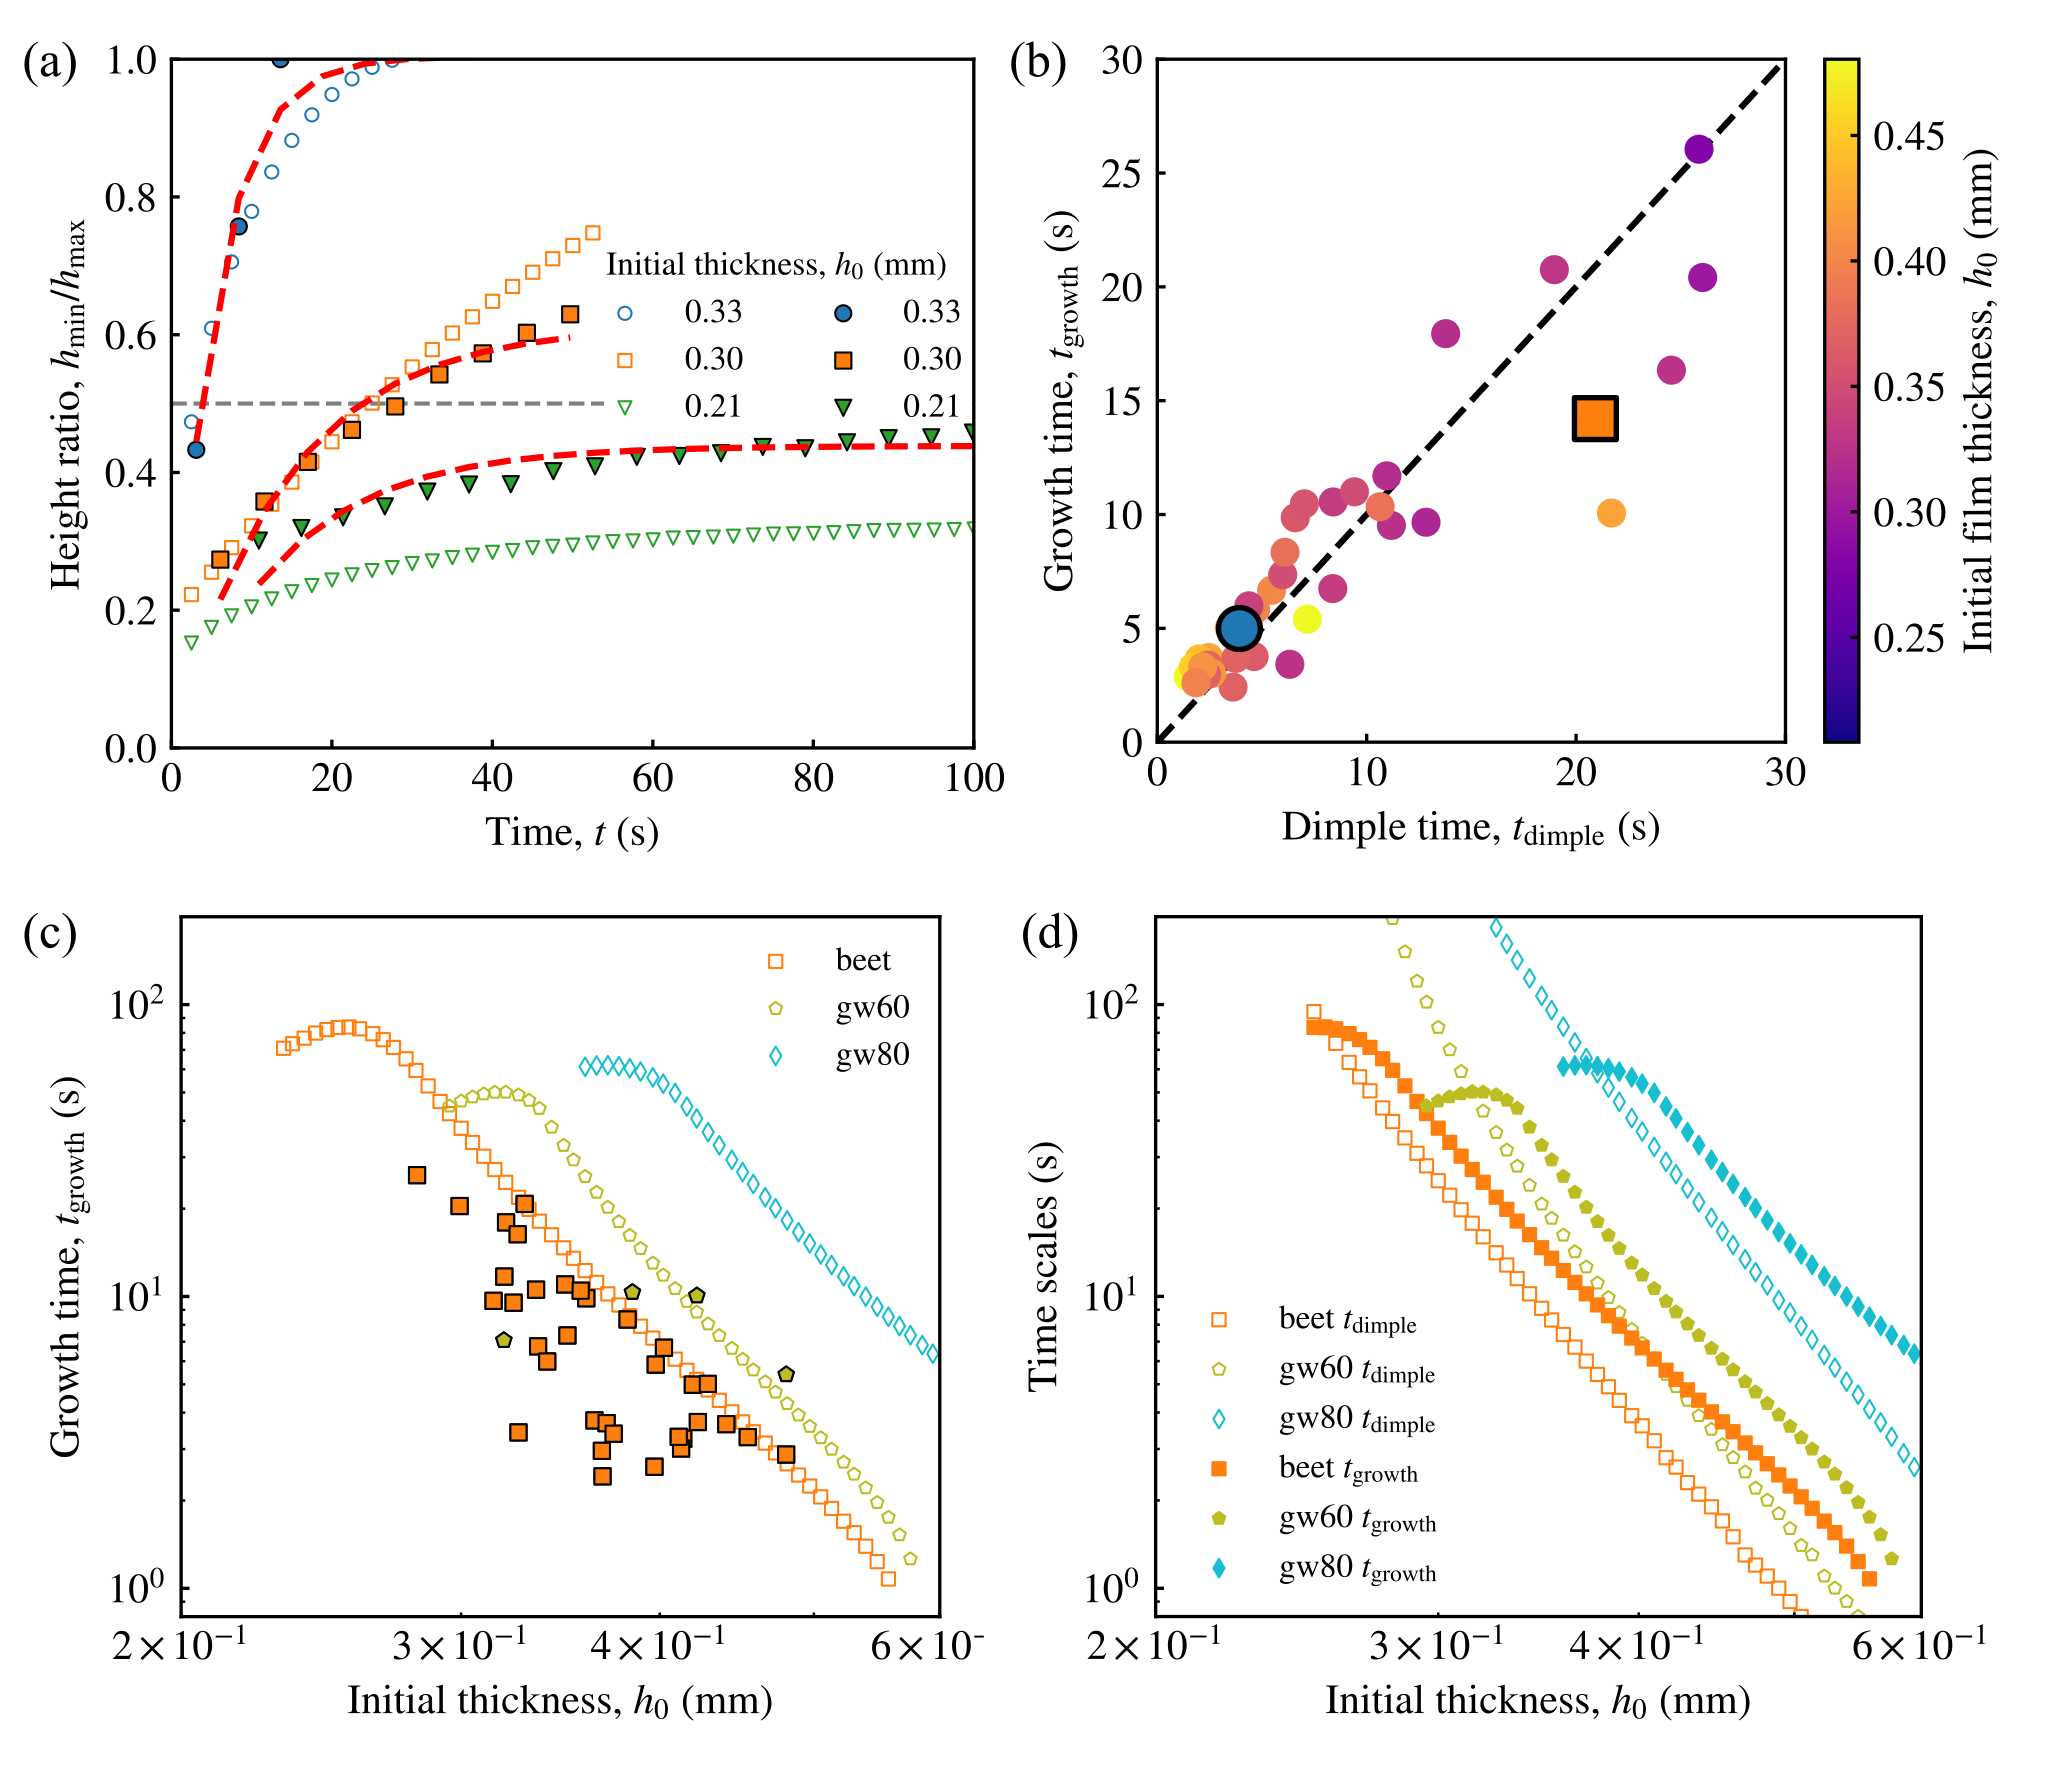
\includegraphics[width=0.8\linewidth]{dimple_growth_time.png}
    \caption{Compare $t_\mathrm{dimple}$ with the alternative time scale $t_\mathrm{growth}$. (a) Temporal evolutions of height ratio (experiment and simulation), fitted by the exponential growth function. (b) Comparison between experimental $t_\mathrm{dimple}$ and $t_\mathrm{growth}$. (c) Experimental and simulated $t_\mathrm{growth}$as functions of initial thickness $h_0$. (d) Comparison between simulated $t_\mathrm{dimple}$ and $t_\mathrm{growth}$ at different $h_0$.}
    \label{fig:dimple-growth-time}
\end{figure}

With this data, this alternative time scale, $t_\mathrm{growth}$, does not rely on arbitrary threshold values, based on the growth rate of the height ratio. Interestingly, this non-arbitrary time scale is quite correlated with the $t_\mathrm{dimple}$ defined in the original text, which does not change the story in this manuscript.

Since $t_\mathrm{growth}$ and $t_\mathrm{dimple}$ behave similarly, and that $t_\mathrm{dimple}$ bears more experimental relevance, we decide to keep using $t_\mathrm{dimple}$ to characterize the dimple relaxation in this work. 

\bigskip
\begin{siderules}
\textbf{Comment 2:} \textit{The scaling plot which could be considered as justification for the above definition is scaled on the vertical axis, but not on the horizontal one. Thus, the collapse observed in the inset of Fig 5d may be completely coincidental.}
\end{siderules}

\textbf{Response:} We thank the reviewer for pointing out the issue with the attempted rescaling shown in the inset of Fig.~5(d) in the original manuscript. 
Our original scaling argument was imcomplete.  
We have revised the scaling argument substantially.

\begin{figure}[ht]
    \centering
    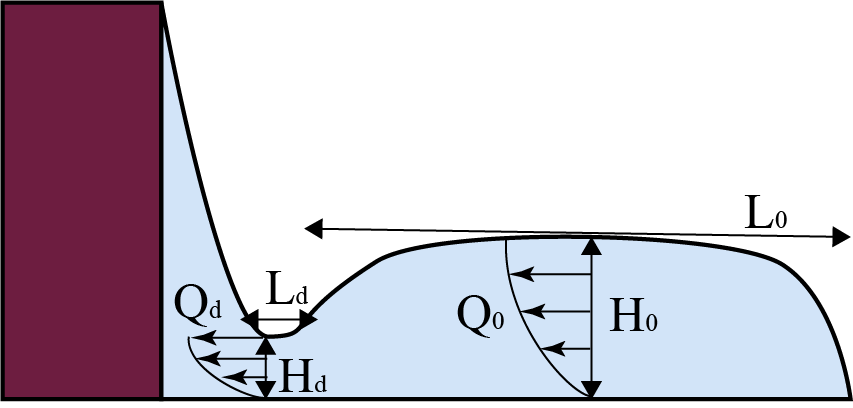
\includegraphics[width=0.4\linewidth]{Responses/rfigs/Schematic.png}
    \caption{Schematic illustrating key variables used in the scaling analysis. }
    \label{fig:Schematic}
\end{figure}



The horizontal velocity is proportional to $ v_x \sim \frac{1}{\mu} \frac{\partial p}{\partial x} z (z- 2h(x))$, and the total flux in a given region is given by $Q \propto \int_0^h v_x dz$. We consider two regions of interest. The flux in the bulk thin film region is 
\begin{equation}
    Q_0 \sim \frac{1}{\mu} \frac{\rho g H_0}{L_0} {H_0^3} \,. 
\end{equation}
The flux through a necking fringe/dimple region is
\begin{equation}
    Q_d \sim \frac{1}{\mu} \frac{\sigma H_d}{L_d^3} {H_d^3} \,. 
\end{equation}
These two fluxes must be equal due to incompressibility.
Assuming that $H_d \propto L_d$ and $H_0 \propto L_0$, one gets 
$H_d \propto H_0^3/\lambda_\mathrm{cap}^2$ where $\lambda_\mathrm{cap} = (\sigma/\rho g)^{1/2}$ is the capillary length. This relation has been confirmed with experimental data as shown below. 

\begin{figure}[ht]
    \centering
    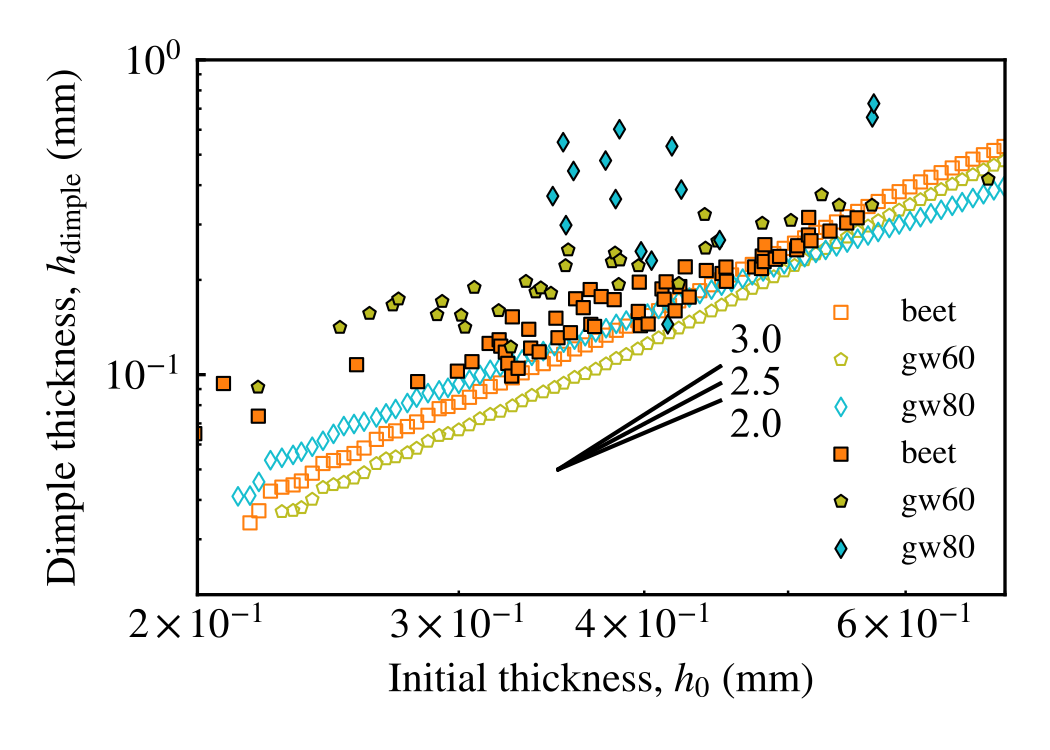
\includegraphics[width=0.4\linewidth]{Responses/rfigs/hh0.png}
    \caption{Compare $h_\mathrm{dimple} (\approx H_d)$ and the initial film thickness $h_0 (\approx H_0)$. The relationship shows that a power-law scaling with an exponent of 3 is a good estimate. }
    \label{fig:h_h0}
\end{figure}

In high Bond numbers, the lubrication time cale is $\mathcal{T} \sim \frac{\mu}{\rho g} \frac{\mathcal{L}^2}{\mathcal{H}^3}$. Here, we assume the characteristic height $\mathcal{H}$ as $H_d$, and length $\mathcal{L}$ as the initial horizontal length $L$. Then, we obtained 
\begin{equation}
    \frac{\mathcal{T}}{\mu \sigma^3 /(\rho g)^4 L^7} \sim \frac{1}{(h_0/L)^9} \,.
\end{equation} 
This relation between non-dimensional time scale and non-dimensional height captures both experimental and simulated data pretty well as shown in Fig. \ref{fig:to_combine}(b). 
The left-hand side scales as $Bo^4 \, Ca^{-1}$, while the right-hand side depends only on the ratio of the characteristic height and length as 
$Bo^4 \, Ca^{-1} \, \frac{\mathcal{T}}{L/V } \sim (h_0/L)^{-9}$. 

\hl{
In the revised manuscript, we wrote details in Section III-E about the scaling arguments and updated Fig. 6. 
}

\begin{figure}[h]
    \centering
    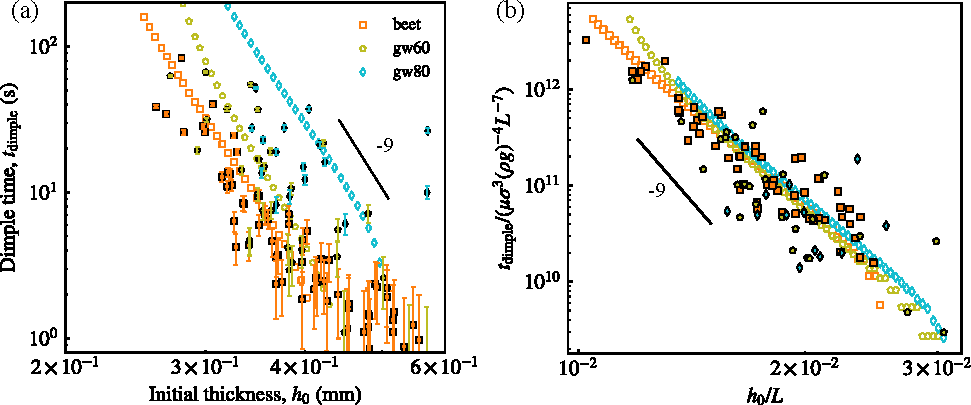
\includegraphics[width=0.8\linewidth]{good_collapse}
    \caption{Compare $t_\mathrm{dimple}$ and non-dimensional $t_\mathrm{dimple}/{\mu \sigma^3 (\rho g)^{-4} L^{-7}}$. (a) Dimple time vs initial thickness. (b) Non-dimensional dimple time vs non-dimensional initial thickness a power-law scaling with an exponent of –9. }
    \label{fig:to_combine}
\end{figure}


\bigskip
\begin{siderules}
\textbf{Comment 3:} \textit{The 100 s “long time” limit is arbitrary, not physically motivated, also Arbitrary.}
\end{siderules}

\textbf{Response:} We thank the reviewer for pointing out the question regarding our choice of time scale. We set the maximum duration of our experiments to 100 seconds to minimize the effect of evaporation. This time duration is approximately an order of magnitude shorter than the evaporation time scale, around 1000 s. 

To estimate the evaporation time scale, we have used the diffusion-limited evaporation rate. The evaporation flux is approximately

\begin{equation}
    J \approx D_v \frac{C_s - C_\infty}{L} 
\end{equation}

where $D_v$ is the diffusion rate of water vapor in air, $C_s$ is the vapor concentration near the surface (saturation), $C_\infty$ is the water vapor concentration far away, and $L$ is the diffusion length scale. Assuming that relative humidity (RH) is 80\%, and diffusion length equals to the film initial thickness $h_0$, we have
\begin{equation}
J \approx D_v \frac{C_s(1-RH)}{h_0}.
\end{equation}
The time it takes to evaporate the beet juice can be estimated as

\begin{equation}
    t_\mathrm{evap} \approx \frac{\rho h_0}{J} \approx \frac{\rho h_0^2}{D_vC_s(1-RH)}.
\end{equation}


Using $D_v=2.5\times 10^{-5}\;\mathrm{m^2/s}$, $C_s=0.023\;\mathrm{kg/m^3}$ and $h_0=3\times 10^{-4}\;\mathrm{m}$, we can estimate the time to be

\begin{equation}
    t_\mathrm{evap} = \frac{1000 \times (3\times 10^{-4})^2}{2.5\times 10^{-5} \times 0.023 (1 - 0.8) } = 782.6\;\mathrm{s}.
\end{equation}


We have modified the text to clarify the reason behind setting 100~s as the cutoff time:

\hl{In terms of the choice of our experiment time, we consider the evaporation time scale. Typically, the evaporation time depends on the relative humidity ($RH$) in the lab. Under a humid condition ($RH = 80\%$), the time for the beet juice to evaporate is estimated as $\approx {\rho h_0}/[D_v {(C_s - C_\infty)}/{L_\mathrm{diffusion}}] \sim {\rho h_0^2}/{(D_vC_s(1-RH))} \simeq 800$ sec. Here, $D_v$ is the diffusion rate of water vapor in the air ($2.5\times 10^{-5}\;\mathrm{m^2/s}$), $C_s$ is the vapor concentration near the surface (saturation; $0.023\;\mathrm{kg/m^3}$), $C_\infty$ is the water vapor concentration far away, and $L_\mathrm{diffusion}$ is the diffusion length scale. Therefore, we chose the maximum duration of our experiments to 100 sec, which is approximately an order of magnitude smaller than the evaporation time ($\mathcal{O} (1000)$ sec).} 


\bigskip
\begin{siderules}
\textbf{Comment 4:} \textit{Fig 5’s caption cites “theoretical model and numerical solutions” but what is shown in a/b are experimental results and numerical simulations;}
\end{siderules}

\textbf{Response:} Sorry for the typo. It is fixed. \hl{``Compare experimental data and numerical solutions.''}

\bigskip
\begin{siderules}
\textbf{Comment 5:} \textit{The experimental technique used is not able to measure the height profile near the solid object in the puddle, so the authors arbitrarily extrapolate with 3rd order with no justification or comment}
\end{siderules}

\textbf{Response:} This work aims to understand the cause of the fringe pattern around a beet slice. We find that the capillary rise on the wall is the key. We characterized the time scale of the dimple. For visualization purpose, we extrapolated the surface profile. However, our key finding, $t_\mathrm{dimple}$ as a function of $h_0$, is independent of the extrapolation. 
	
We further emphasize this in the revised manuscript:

\hl{
This extrapolation is not an accurate account for the meniscus shape, and is done only for presenting the meniscus shape more realistically. The key finding $t_\mathrm{dimple}$ of this work does not rely on the extrapolated data.
}

\bigskip
\begin{siderules}
\textbf{Comment 6:} \textit{Fig 5’s caption cites “theoretical model and numerical solutions” but what is shown in a/b are experimental results and numerical simulations;}
\end{siderules}

\textbf{Response:} Sorry for the typo. It is fixed. \hl{``Compare experimental data and numerical solutions.''}

\bigskip
\begin{siderules}
\textbf{Comment 7:} \textit{Fig A3 is for data “around” 6 seconds,}
\end{siderules}

\textbf{Response:} We thank the reviewer for pointing out the unclear writing. We have revised the scaling argument substantially. \hl{Fig.A3 is no longer needed and is now removed.}

\bigskip
\begin{siderules}
\textbf{Comment 8:} \textit{Appendix E shows the influence of “all” the parameters,}
\end{siderules}

\textbf{Response:} We thank the reviewer for pointing out the unclear writing. We have rephrased it to ``the influence of surface tension, viscosity, initial thickness and film length''. In addition, we measured the dimple time at various surface tension, viscosity, initial thickness and film length to assess the effects of these parameters. Some insight into the role of the film length is provided (see the revised \hl{Appendix G}).

\bigskip
\begin{siderules}
\textbf{Comment 9:} \textit{the discussion in Appendix F is too superficial,}
\end{siderules}

\textbf{Response:} We thank the reviewer for pointing this out. 

As is mentioned in our response to Comment 2, we have revised the understanding of the time scale substantially. 
\hl{The original Appendix~F is now removed, and an in-depth discussion on $t_\mathrm{dimple}$ is presented in Section~III~E in the revised manuscript.}


\bigskip
\begin{siderules}
\textbf{Comment 10:} \textit{Appendix G refers to “my” scaling.}
\end{siderules}

\textbf{Response:} We rephrase it to \hl{``the scaling (Eq.~2)''}.

\end{document}
